\section{Offline Selections and Analysis of the Data}

In this analysis we search for evidence of new light bosons decaying into pairs of muons. The new particles can be isolated or produced in groups, coming from cascade decays in the new sector ending with several instances of the lowest-state particle. In addition to di-muon decays, the new particle decay channels can include pairs of electrons and perhaps hadrons. In many scenarios, multiple instances of such new boson can be produced per event. This analysis is therefore searching for one of more pair of muons with the invariant mass consistent with being produced in the decays of the same particle. Assuming on-shell production of at least a fraction of these new bosons per event, the new physics would manifest itself as enhancement in the rate of production of muon pairs consistent with a certain common mass. 

We attempt to achieve a balance of two important goals. First, to achieve high sensitivity for a representative range of specific new physics scenarios leading to characteristic muon jet signatures and, second, to present results that would allow future interpretation in the context of other models of new physics yielding lepton jet signatures. Essentially all classes of models of new physics relevant to this analysis lead to the production of events of several different topologies in terms of the number of collimated muon jets and multiplicities of muons within each jet. Because these topologies have different sources and levels of SM backgrounds, we categorize events using topologies with different expected signal-to-background ratios to maximize the overall sensitivity of the analysis. Achieving the second goal requires minimal dependence of acceptance on the details of a specific model, which often arise due to detector inefficiencies that can be difficult to parameterize in a fully generic way. 

In the offline analysis, events are required to have at least one primary vertex 
reconstructed in the  luminous region along the beamline to minimize background events not originating 
from collisions. Selected events are 
further required to have at least one high quality muon candidate with $p_T>15$~GeV/$c$ 
matching the muon selected in the online trigger and within $|\eta|<0.9$ reconstructed using 
an inside-out algorithm, which ensures high efficiency in the environment with multiple nearby muons. 
This algorithm extrapolates tracker tracks into the muon system and attaches individual tracklets (stubs) 
reconstructed in muon chambers. The assignment is arbitrated in the sense that any stub in the muon 
system can only be associated with one extrapolated tracker track most compatible with the stub. The 
reconstructed muon candidate is required to have stubs in at least two out of four muon stations it crosses. To 
be classified as high-quality, muon candidates are required to have at least eight hits in the silicon tracker. The 
requirement of $|\eta|<0.9$ is necessary to ensure high and well understood trigger 
efficiency insensitive to the presence of muon hits from other nearby muons
expected in the signatures with collimated muons. It avoids the endcap region where trigger 
efficiency can be substantially diminished in the presence of multiple closely spaced muons due to the features of 
the trigger electronics setup. Additional muon candidates are required to have $p_T>5$~GeV/$c$, to be contained 
within $|\eta|<2.4$, and to satisfy the same quality requirements.

Muon jets are reconstructed by iteratively clustering muon candidates starting with one of the muon
candidates. Each additional muon is added to the jet if the invariant mass of the new muon and any
opposite charge muon already assigned to the jet satisfies $m(\mu,\mu)<9$~GeV/$c^2$ and is
compatible with originating from the same vertex (confidence level of the vertex fit $>$ 1\%). This clustering procedure always converges and is 
independent of the order in which muons are added to muon jets. The choice of $m(\mu,\mu)<9$~GeV/$c^2$ ensures that muons originating from the same $b$-quark are always clustered into the same muon jet and most muons originating from different $b$-quarks are clustered into different muon jets.  It is also appropriate 
for topologies predicted by most relevant models of new physics, as the typical masses of the heavier 
hidden states originating the cascades are of the order of a few GeV/$c^2$. Note that the efficiency of the 
clustering algorithm does not depend on the boost of the muon jets, thereby reducing the sensitivity of the analysis 
to the details of the kinematics that can differ from one model to another. As a consequence of the clustering algorithm, each muon jet must contain at least one muon of each charge, but can contain arbitrarily many muons. 
Within each muon jet, we identify the pairs of muons that are most likely to have arisen from individual dark photon decays by assigning pairs of oppositely charged muons with minimal difference in dimuon mass (since all instances of the dark photon have the same mass).  We refer to such pairs as fundamental dimuons.

All events are then categorized according to the number of muon jets $N$ and the number of muon candidates $n_i$ in the $i^{\mbox{\scriptsize th}}$ muon jet, thus forming topologies denoted as $R^{N}_{n_1 ... n_N}$. In topologies with multiple dimuon candidates, the reconstructed masses of all fundamental dimuons would be consistent with each other within detector resolution for signal events, but not necessarily for backgrounds. Therefore, we build a $K$-dimensional distribution of reconstructed dimuon masses $m_1, ..., m_K$ for each topology, where $K$ is the number of reconstructed dimuons per event. The signal of new physics would appear as a striking enhancement of events at a point near the $K$-dimensional diagonal with $m_1 \sim ...\sim m_K \sim m_0$, where $m_0$ is the mass of the new particle. While the distributions of background events are not smooth due to low-mass resonances, the background distributions extend beyond the diagonal in a known way. If such enhancement were to be observed, one can further construct the invariant mass of combinations of dimuons in the same muon jet to search for possible structure, e.g.\ a process of the type $a_2 \to a_1 a_1 \to (\mu\mu) (\mu\mu)$ would lead to an enhancement in the invariant mass of pairs of dimuons consistent with $m(a_2)$. The only exception is the $R^1_2$ topology with exactly one fundamental dimuon per event: the signal would appear as a narrow peak in the 1D distribution of dimuon mass $m$. For topologies with $K$ dimuon candidates, we define the signal region as a ``corridor'' near the diagonal in the $K$-dimensional space of width $5 \times \sigma(m)$, where $\sigma(m) = (0.026 + 0.0065\, m )$~GeV/$c^2$ (for barrel $|\eta^{\mu\mu}| < 0.9$) and $(0.026 + 0.013\, m )$~GeV/$c^2$ (for endcap $0.9 < |\eta^{\mu\mu}| < 2.4$). The parameterization for $\sigma(m)$ was derived from studies of $J/\psi$, $\psi'$, $\phi$, $\rho/\omega$, and $\eta$ (decays to $\mu \mu \gamma$) resonances and high-$p_T$ Monte Carlo simulations, and corresponds to the resolution expected of hypothetical dimuons with $p_T\sim300$~GeV/$c$ in the barrel region and $p_T\sim 150$~GeV/$c$ in the endcap. After the shape of the background events distribution in the $K$-dimensional space is measured, the data in the off-diagonal part can be used to obtain the background normalization, which can then be used to fit the data in the near-diagonal region for signal plus background.

\begin{figure}[tbh]
\centering
\begin{tabular}{cc}
\includegraphics[width=0.45\linewidth]{fig/template__bkg_model_a1__m_1_log.pdf} &
\includegraphics[width=0.45\linewidth]{fig/template__bg_sh_b1t__m_1_log.pdf} \\
\includegraphics[width=0.45\linewidth]{fig/template__bg_sh_b1o__m_2_log.pdf}&
\includegraphics[width=0.45\linewidth]{fig/template__bg_sh_a2_02_1__m_1_log.pdf}\\
\includegraphics[width=0.45\linewidth]{fig/template__bg_sh_a2_02_2__m_2_log.pdf}&
\includegraphics[width=0.45\linewidth]{fig/template__bg_sh_a2_11_1__m_1_log.pdf}\\
\end{tabular}
\caption{Dimuon invariant mass distributions in the background-enriched samples for different topologies. The data are overlaid with parameterized functions, fitted to the data. These are used to construct mass-shape templates for the distributions of background events in signal regions. Background templates for topologies with high muon multiplicity are modeled as Cartesian products of these distributions.  (a): Distribution of the single-dimuon events (topology $R^1_2$) with $40<p_T^{\mu \mu}<60$~GeV/$c$.  (b): Distribution of dimuon events containing a trigger-quality muon ($p_T>15$~GeV/$c$ and $|\eta|<0.9$) used to model the invariant mass shape of the ``first'' dimuon candidate in the two-dimuon topology $R^2_{22}$.  (c): Dimuon invariant mass distribution for events with a dimuon candidate and an additional, unclustered, trigger-quality muon, used to model the distribution of the ``second'' dimuon in background events in topology $R^2_{22}$.  (d), (e) and (f): Distributions of the ``dimuon'' invariant mass in events with two muons and two tracks playing the role of misidentified muons in quadmuon topology $R^1_4$, for the cases when the dimuon is reconstructed from two true muons, one true muon and a track, and two tracks emulating misidentified muons, respectively. 
\label{fig:background_distributions}}
\end{figure}

Event topologies $R^{N}_{n_1 ... n_N}$ have different rates and compositions of the SM backgrounds. The single-dimuon topology $R^1_2$ suffers from a particularly high rate of the SM backgrounds due to $b\bar{b}$ and Drell-Yan processes. Without additional selections, the SM backgrounds would be too large to maintain sensitivity to signals with picobarn-scale cross-sections. To reduce the SM backgrounds, events in the $R^1_2$ topology are additionally required to have a substantial transverse momentum of the muon jet $p_T^{\mu\mu}>80$~GeV/$c$. This requirement dramatically improves the sensitivity of this topology for new physics signals that predict highly boosted muon jets. At the same time this requirement reduces acceptance for signal events containing only one dimuon per event, particularly for models with lower boosts of muon jets. For such models the sensitivity is driven by events in topologies with two or more dimuons per event, for which no high momentum requirement is imposed. Data events in topology $R^1_2$ with lower momentum dimuon candidates are used for background studies and validation of the background estimation techniques. 

The only criteria used to identify and categorize signal topologies, other than the high-momentum requirement applied to $R^1_2$, are the number of muon jets and the number and charge of muons within each muon jet.  Muons that do not belong to any muon jet (which may arise from SUSY cascades, rather than dark photon decay) are neither used to identify nor to reject signal events.  Other reconstructed objects, such as hadronic jets and missing energy, are neither selected nor rejected, even implicitly as an isolation cut.  Of all possible combinations of $N$ and $n_i$, only $R^1_3$, with low expected signal content, is not considered a signal.  It is instead used as a control to test background parameterizations.

The background rates in the selected topologies are expected to be low with the exception of topology $R^1_{2}$, where backgrounds remain not negligible even after the $p_T^{\mu\mu}>80$~GeV/$c$ requirement. However, because the search for new resonances is performed in small windows in the invariant mass distribution of muon pairs, the rate of remaining background events in each window is at the level of a fraction of 1~pb, comparable to the rate of the signal if it is present in data. For topology $R^1_2$, the main SM background contributions are due to $b\bar{b}$ production with one of the $b$-quarks undergoing a double semi-leptonic decay, low-mass resonance production (prompt or from heavy flavor decays), low-mass Drell-Yan production, and occasional muon misidentifications due to decays-in-flight, either alone or in combination with a muon from the heavy flavor.  For topology $R^2_{22}$, the SM backgrounds are dominated by the $b\bar{b}$ production with both $b$-jets undergoing double semileptonic decays or fragmenting into low-mass resonances decaying to pairs of muons. Background events with muon jets consisting of multiple muon candidates (``quadmuon'' topology $R^1_{4}$ and the higher order topologies) typically originate from events with two muons from a $b$-jet and the other muons from either decays-in-flight, punch-through, or muon misidentifications where some of the segments from true muons are matched to the non-muon tracks. The SM content of the higher order regions is due to rare combinations of the causes discussed above and is extremely low. 

\begin{figure}[tbh]
\centering
\begin{tabular}{cc}
\includegraphics[width=0.45\linewidth]{fig/template_control__bkg_model_a1__m_1_log.pdf} &
\includegraphics[width=0.45\linewidth]{fig/template_control__bkg_model_b1.pdf}\\
\includegraphics[width=0.45\linewidth]{fig/template_control__bkg_model_a2__m_1.pdf} &
\includegraphics[width=0.45\linewidth]{fig/template_control__bkg_model_a2_inv__m_inv_log.pdf} \\
\end{tabular}
\caption{
(a): Data in the single-dimuon category ($R^1_2$) control region $60<p_T^{\mu\mu}<80$~GeV/$c$ overlaid with the background prediction obtained from the background-enriched region $40<p_T^{\mu\mu}<60$~GeV/c, fitted for overall normalization only. 
(b): The invariant mass of all dimuons in the off-diagonal region for events in the two-dimuon category ($R^2_{22}$, note that there are two entries per event), compared with the prediction obtained from the full 2D background template, fitted for overall normalization only.
(c): The invariant mass distribution of all ``dimuons'' in the $3\mu+$track events (two entries per event) used as a control region for the analysis of events in the quadmuon category ($R^1_4$). The distribution is compared with the prediction obtained from the full 2D background template, fitted for overall normalization only. 
(d): The invariant mass of of the four ``muons'' in the $3\mu+$track control region for the quadmuon topology $R^1_4$ compared with the prediction obtained from the data in the background-enriched region ($2\mu+2$tracks).
\label{fig:control_distributions}}
\end{figure}

To account for background contributions, we construct templates (one for each topology) modeling the distribution of reconstucted muon pair masses in background events. With the exception of the single dimuon topology $R^1_2$, the templates are multi-dimensional distributions in the $(m_1, ..., m_K)$ space of reconstructed muon pair masses, where $K$ is the number of dimuons characteristic of a given topology. 
For each category, we define one or more background-enriched regions used to construct the template. In addition, we define a control region for validating the template using events with properties closely resembling those of the final events or using the off-diagonal side-band of the final $(m_1, ..., m_K)$ distribution. 

While the templates were derived directly from data, we use simulation to determine the composition of the backgrounds as well as momentum evolution of certain parameters, e.g.\ the dimuon mass resolution and shape of the invariant mass distributions. To ensure 
that simulation is reliable in the phase space characteristic of this analysis, a series of detailed studies have been performed. First, the single-dimuon dataset with $p_T^{\mu \mu}<80$~GeV/$c$ (low momentum part of topology $R^1_2$) was divided in subsets dominated by one of the each contributing background prcocesses to measure rates, shapes, kinematic distributions, tracking related parameters and resolutions, mass resolutions of low-mass resonances as a function of boost, etc. These measurements were compared to simulation predictions showing very good agreement except a few known and well-understood shortcomings of the available simulated samples (lack of very low-mass Drell-Yan, missing production modes and/or dropped decay channels for some resonances).

To model the shape of the invariant mass distribution for the single dimuon region $R^1_2$, we define two sub-regions with $40<p_T^{\mu \mu}<60$ (background enriched region) and $60<p_T^{\mu \mu}<80$~GeV/$c$ (control region). The first sub-region is used to obtain a parametrization of the shape of the dimuon invariant mass distribution in background events shown in Fig.~\ref{fig:background_distributions}(a). To validate the template, we fit its shape (with the resolution of mass measurement evolved to higher $p_T^{\mu\mu}$) to the observed data in the sub-region $60<p_T^{\mu \mu}<80$~GeV/$c$, allowing only the overall normalization to float in the fit. The comparison shows good agreement as illustrated in Fig.~\ref{fig:control_distributions}(a). The same template (with mass resolution evolved to even higher $p_T^{\mu\mu}$) is used to predict the shape of background events of topology $R^1_2$ in the signal region $p_T^{\mu\mu}>80$~GeV/$c$.

The SM backgrounds in the two-dimuon topology $R^2_{22}$ are dominated by $b\bar{b}$ events with each $b$-quark yielding a pair of muons. Because each $b$-jet fragments independently, the background distribution in the $(m_1,m_2)$ space of the two dimuon masses is a Cartesian product of the 1D dimuon mass distribution with itself. However, because one of the dimuons contains the $p_T > 15$~GeV/$c$ muon that triggered the event, its dimuon mass spectrum is different from that of the other dimuon. To acount for this effect, we separately measure the shapes for the ``trigger'' and non-trigger dimuons. To model the ``trigger dimuon'' shape, we use single-dimuon events with further selections suppressing the non-$b\bar{b}$ backgrounds, fit to a parameterized functional form, subtracting residual contamination from Drell-Yan (both subtracted and non-subtracted curves are shown in Fig.~\ref{fig:background_distributions}(b)). To match the kinematics of the two-dimuon events being modeled, the ``other dimuon'' shape is obtained using three-muon events with a dimuon recoiling off a trigger-quality muon and is shown in Fig.~\ref{fig:background_distributions}(c). To properly account for a contribution with both dimuons containing a trigger-quality muon in the final 2D template, an additional re-weighing is applied in taking the Cartesian product of the two distributions. The template is validated using final two-dimuon events in the off-diagonal part of the $(m_1,m_2)$ distribution. Figure~\ref{fig:control_distributions}(b) shows a comparison of the invariant mass distribution of the dimuons in these events (note that there are two histogram entries per event), compared to the prediction derived from the template and fit to the data for overall normalization only. 

The quadmuon topology $R^1_4$ has a small background contamination in which a $b$-quark produces two real muons and an additional two muons are produced from from non-muon tracks incorrectly matched to some of the real muons' stubs. When identifying the two fundamental dimuons within the group of four muons, both $(\mu , \mu)+(trk ,trk)$ and $(\mu ,trk)+ (\mu, trk)$ pairings can occur, each having its own distinct 2D shape in the $(m_1,m_2)$ space. To model these events, we use single dimuon events and construct ``pseudo mu-jets'' using two reconstructed muons and two non-muon tracks playing the role of misidentified muons. Selected events are separated into two subsets according to the type of pairing, each producing a 2D distribution for the invariant masses of the two pairs in the event. Figures~\ref{fig:background_distributions}(d), (e) and (f) show 1D invariant mass distributions for $(\mu , \mu)$, $(trk ,trk)$, and $(\mu ,trk)$-type dimuons obtained from projections of the 2D distributions for the two types of events. In the $R^1_4$ signal events, the identities of $\mu$ and $trk$ are unknown, so the mass templates and the signal events are both symmetrized by randomly assigning dimuon masses to the horizontal and vertical axes of the plot. The template is validated using a control region with three nearby muon candidates ($R^1_3$), one of which is likely a misidentified hadron, and adding a non-muon track to play the role of a second misidentified muon. Figure~\ref{fig:control_distributions}(c) compares the distribution of all ``dimuons'' in the $3\mu+$track control sample (note two entries per event) compared to the prediction based on the full 2D template fitted to data for overall normalization only. Figure~\ref{fig:control_distributions}(d) makes a similar comparison but for the quadmuon invariant mass. Templates for higher order topologies are derived as combinations of the above methods. In all cases, the full posterior density functions for fit parameters including correlations were saved to be used in the final fit to account for the uncertainties in the background templates.

\begin{figure}[tbh]
\centering
\begin{tabular}{cc}
\includegraphics[width=0.4\linewidth]{fig/sig_data_bg_a1.pdf} & 
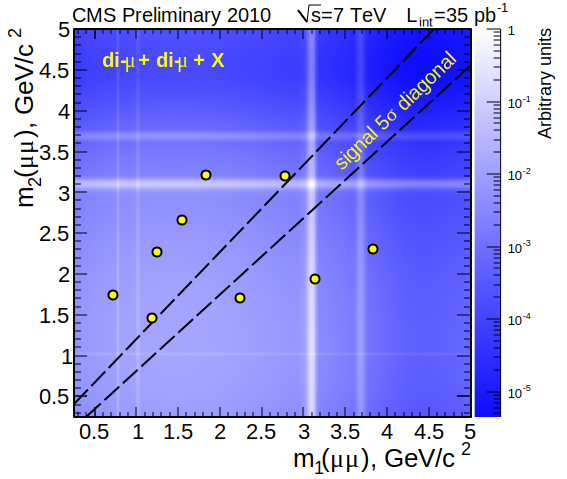
\includegraphics[width=0.4\linewidth]{fig/sig_data_bg_b1.pdf} \\
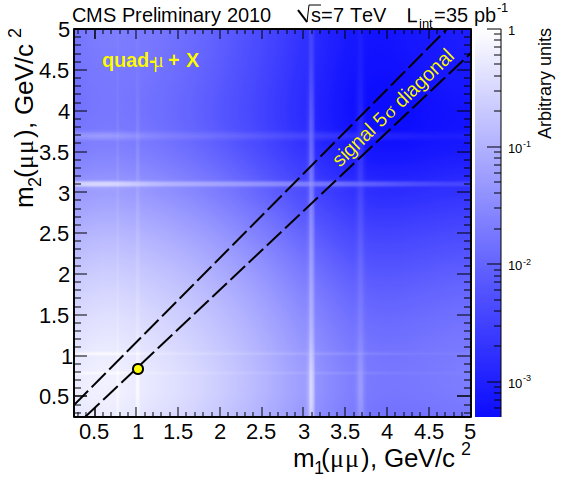
\includegraphics[width=0.4\linewidth]{fig/sig_data_bg_a2.pdf} & 
\includegraphics[width=0.4\linewidth]{fig/sig_data_bg_a2_inv.pdf}\\
\end{tabular}
\caption{2D and 1D invariant mass distributions of muon pairs for events in each signal region, compared with the expected background: ``single dimuon'' events in topology $R^1_2$ (a), 10 events in the ``two-dimuon'' topology $R^2_{22}$ (b), the single ``quadmuon'' event in topology $R^1_4$, (c) and the invariant mass of all four muons for the same event (d). None of the events in the the multi-dimensional topologies fall into the corridor along the diagonal (shown as dashed lines), which would indicate the presence of signal. The last plot is relevant for the special scenario with a cascade decay $a_2 \to a_1 a_1$ with $m(a_2)<2 m(a_1)$, leading to the off-shell production of $a_1$. \label{fig:signal_distributions}}
\end{figure}

As mentioned above, the shapes of the invariant mass distribution for signal events was studied by comparing the properties of events with dimuons from $\omega$, $\phi$, $J/\psi$ and $\psi^{\prime}$ resonances in data with the simulation predictions and extrapolating between the resonance masses. Because of the excellent resolution of the CMS tracker, signal shapes have narrow width scaling with the mass of the resonances, with a slight dependence on the dimuon transverse momentum. For final fits, signal shape is parameterized using a Crystal Ball function with core resolution of $\sigma(m) = (0.026 + 0.0065\, m )$~GeV/$c^2$ (for barrel $|\eta^{\mu\mu}| < 0.9$) and $(0.026 + 0.013\, m )$~GeV/$c^2$ (for endcap $0.9 < |\eta^{\mu\mu}| < 2.4$). Multi-dimensional distributions were obtained by taking appropriate Cartesian products. The uncertainties on the parameters of the function are obtained by quantifying the level of agreement between data and simulation, which is dominated by the statistical uncertainties due to the size of samples reduced by the requirement of an appreciable boost. For dimuons with $p_T^{\mu\mu}<150$~GeV/$c$, the reconstruction efficiency in the barrel region is nearly flat, is on average $95 \pm 1$\%, and is driven by the efficiency in the finding and matching stubs in the muon system. The efficiency decreases to about 92\% for $m(\mu\mu)$ close to $2m_\mu$ due to muon trajectories becoming nearly collinear. In the endcap region, there is a slight lowering of efficiency towards high $|\eta|$ due to muon trajectories overlapping in the muon system. The systematic uncertainty on the efficiency in he endcap region is 3\%. For higher-momentum dimuons, tracking effects become important as the overlaps of the trajectories leads to high sharing of hits and decreased efficiency. The effect is especially pronounced for $m(\mu\mu)$ of 0.4--0.6 GeV/c$^2$, where the efficiency decreases to $85\pm 5$\% at $p_T^{\mu\mu}\sim 250$~GeV/$c$ and to $75\pm 10$\% at $p_T^{\mu\mu}\sim 350$~GeV/$c$ due to ``cowboy''-type events, in which muon trajectories bend towards each other in the magentic field and remain close to each other for a substantial part of their paths through the tracker. For muon pairs with $m(\mu\mu)$ outside of this range, the efficiency is nearly flat until 250~GeV/c$^2$, where it starts a slow descent towards higher momentum, being about $85\pm5$ at $p_T(\mu\mu)\sim350$~GeV/$c$. The above-quoted uncertainties account for possible inaccuracies in modeling the size of the tracker hit clusters in the silicon tracker, which could affect the rate of merging hits from nearby tracks, driving the inefficiency of track reconstruction.

Reconstruction of quadmuons, e.g.\ produced via $h_d \to \gamma_d \gamma_d \to 4 \mu$, suffers more significantly from reconstruction failures in the muon system. In addition to the 3\% inefficiency per muon, quadmuon efficiency has a significant additional term related to small uninstrumented gaps beween the wheels of the muon system. With an inefficiency of 8--10\% per muon crossing the gap region and a significant probability for one or more muons to cross it, the average reconstruction efficiency for a quadmuon is $83\pm 3$\%. For high-momentum quadmuons, where tracking effects become more significant, the efficiency is determined by the probability to reconstruct each of the two low-mass dimuons comprising the quadmuon as the overlaps of muons from different dimuons are rare. Momentum dependence of the quadmuon efficiency closely follows the reconstruction efficiency of a dimuon with momentum equal to the higher-momentum dimuon within the quadmuon. It also has the same dependency on the invariant mass of the dimuons within the quadmuon. For a quadmuon with constituent dimuon mass of about 0.5~GeV/c$^2$ (the worst-case scenario), the average efficiency at $p_T^{\mu\mu\mu\mu}\sim350$~GeV/$c$ is about 76\% and has a systematic uncertainty of 2--3\% due to the tracking effect. Higher-multiplicity muon jets have larger inefficiencies due to muon system reconstruction failures, but would be reconstructed as lower-multiplicity jets. In the context of a specific model, the migration of events between the high-multiplicity topologies does not reduce the overall acceptance. Higher-multiplicity muon jet reconstruction is less affected by tracking inefficiencies as the average momentum of dimuons is moderate, even for very high momentum ($p_T^{\mu-jet}>400$~GeV/$c$) muon jets.

\section{Results}

The data in the regions used to search for signal (the ``diagonal'' regions of multi-dimensional distributions and the single-dimuon events with $p_T^{\mu\mu}>80$ GeV/c) were hidden from the analyzers until all analysis selections and signal extraction techniques were finalized. When the signal regions were revealed, no evidence of new resonance production was found within the sensitivity of this analysis. Figure~\ref{fig:signal_distributions} shows the observed data for select topologies and the expted SM background contributions, which were obtained using the templates for each topology.  The templates were normalized to the data in the off-diagonal regions in high-multiplicity topologies (all but $R^1_2$) and directly fitted in a combined signal-plus-background fit for the single-dimuon case ($R^1_2$). No events were found in any topologies with more than four muons.

To interpret the results in a model-independent fashion, we set the 95\% C.L. upper limits on the alowed production rate of single-dimuon+X, quadmuon+X and two-dimuons+X topologies. The rate is defined as the cross-section times appropriate branching fractions to produce a particular signature times kinematical and geometrical acceptance (muon momentum thresholds and $\eta$ ranges), assuming an ideal detector. Limits are set using Bayesian technique including integration over the systematic uncertainties in the signal and background shape parameterizations and the background normalization, which are treated as nuisance parameters. The limits shown in Fig.~\ref{fig:final_limits} account for instrumental inefficiencies as well as variations in reconstruction efficiencies for dimuon masses ranging from $0.25$ to 5~GeV/$c^2$ and the mean of the muon jet (dimuon or quadmuon) momentum distributions up to 250~GeV/$c$. These variations were treated as an additional systematic uncertainty and were 7\% for the quadmuon topology, 20\% for dimuon, and 35\% for two dimuon topology. For higher momentum muon jets, the limits would become weaker due to diminishing reconstruction efficiency. Other systematic uncertainties account for the accuracy in the luminosity measurement (4\%), uncertainties in the efficiency of reconstructing and matching muon stubs to the tracks and triggering (1-4\% depending on the topology), and track reconstruction efficiency (5-10\%). The presented quadmuon+X limit can be used as a lower bound on signals with muon jets containing four or more muons in it. Note that these limits are conservative in the sense that they assume that reconstruction failures always exclude events from consideration while in realistic models reconstruction failures cause events to be reconstructed in one of the lower multiplicity topologies. 

\begin{figure}[tbh]
\centering
\begin{tabular}{cc}
\includegraphics[width=0.45\linewidth]{fig/ul__model_indep_sys.pdf} &
\includegraphics[width=0.45\linewidth]{fig/ulimit_model_u1.pdf}\\
\includegraphics[width=0.45\linewidth]{fig/ulimit_model0.pdf} &l
\includegraphics[width=0.45\linewidth]{fig/ulimit_model1.pdf}\\
\end{tabular}
\caption{(a) 95\% C.L. upper limits on the rate of the signals of new physics with lepton jets for three topologies. (b) Limits for the Dark SUSY model with the MSSM LSP decaying via $\tilde{\chi}^0_1 \to \tilde{\chi}_d \gamma_d+\tilde{\chi}_d h_d (\to \gamma_d \gamma_d)$, with the $\tilde{\chi}_d$ being the cold dark matter candidate (c) and (d): limits on the model where squark is the MSSM LSP decaying into a quark and a light hidden sector fermion decaying to a lighter hidden sector fermion with emission of either a dark photon or a light dark higgs decaying to two dark photons. 
\label{fig:final_limits}}
\end{figure}

To set limits for representative benchmark scenarios, we use two models for SUSY with the dark sector. The first SUSY model~\cite{BaiHan} assumes standard MSSM squark/gluino production and cascades followed by the decay of the MSSM LSP into the dark sector $\chi_1^0 \to h_{\mbox{\scriptsize dark}} \chi_{\mbox{\scriptsize dark}}$ or $\chi_1^0 \to \gamma_{\mbox{\scriptsize dark}} \chi_{\mbox{\scriptsize dark}}$, where $\chi_{\mbox{\scriptsize dark}}$ is the new cold dark matter candidate. The dark sector masses used are $m(h_{\mbox{\scriptsize dark}})=3$, $m(\gamma_{\mbox{\scriptsize dark}})=0.5$, and $m(\chi_{\mbox{\scriptsize dark}}=300$~GeV/$c^2$. The resulting limits are shown as a function of gluino mass $m(\tilde{g})$ ($m(\tilde{q})=m(\tilde{g})/1.2$ for first two generations) in Fig.~\ref{fig:final_limits}(b) for three different choices of branching fractions $B(\gamma_{\mbox{\scriptsize dark}} \to \mu \mu)$. In addition to the systematic uncertainties used for model-independent limits, we include the uncertainty of 3\% in the acceptance to account for uncertainties in PDFs by varying parameterizations within the CTEQ6.6~\cite{cteq6} family, and comparing central values of CTEQ6.6L with  NNPDF2.0~\cite{nnpdf}, and MSTW2008~\cite{mstw} sets).
The second model~\cite{Ruderman} assumes squarks to be the standard MSSM LSP ($m(\tilde{q})=m(\tilde{g})/1.2$). Following production, squarks decay via $\tilde{q} \to q n_2$, where $n_2$ is a heavier dark sector fermion with the decay modes dominated by either $n_2 \to n_1 \gamma_{\mbox{\scriptsize dark}}$ or $n_2 \to n_1 h_{\mbox{\scriptsize dark}}(\to \gamma_{\mbox{\scriptsize dark}}\gamma_{\mbox{\scriptsize dark}})$. For each of the two sub-models the limits on the production cross-section are shown in Fig.~\ref{fig:final_limits} (c) and (d) for three different choices of branching fractions $B(\gamma_{\mbox{\scriptsize dark}} \to \mu \mu)$. The dark sector masses are set to $m(h_{\mbox{\scriptsize dark}})=1.2$, $m(h_{\mbox{\scriptsize dark}})=0.5$, $m(n_2)=2$, $m(n_1)=0.5$~GeV/$c^2$. The cross section curves shown in Figs.~\ref{fig:final_limits}(b-d) assume universality of squark masses across all three generations and therefore can be substantially lower if those are not universal. These limits are the most stringent limits for models with dark SUSY sector from collider experiments.

\begin{figure}[tbh]
\centering
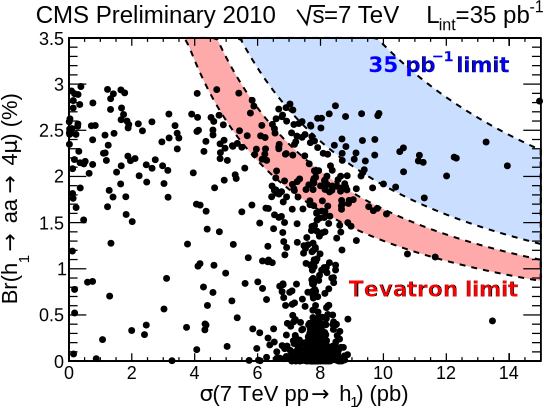
\includegraphics[width=0.45\linewidth]{fig/limits_on_models_7tev.pdf}
\caption{The NMSSM models consistent with WMAP and LEP higgs constraints (shown as points) compared to the exclusions obtained by setting a 95\% C.L. upper limits on the higgs production via the $h_1 \to a_1 a_1 \to 4 \mu$ channel in this analysis and in the Tevatron searches. Both searches exclude the upper right corner of the parameter space, exclusion limits depend on the exact masses of $h_1$ and $a_1$ and therefore are shown as bands corresponding to $m{h_1}$ varied from 89 to 120 GeV/c$^2$ and $m(a_1)$ varied from $2m(\mu)$ to $2m(\tau)$. 
\label{fig:nmssm_limits}}
\end{figure}

Finally, we consider a model with the NMSSM higgs production decaying via $h_1 \to a_1 a_1$. If $m(a_1)<2m_\tau$, $a_1$ has a significant branching fraction for decays into a pair of muons. The sensitivity of this analysis to $\sigma(pp) \to h_1 \to a_1 a_1 \to (\mu\mu) (\mu\mu)$ is dominated by the two-dimuon region $R^2_{22}$ leading to a 95\% C.L.\ limit on the production rate of about 0.2~pb. To interpet the limit in the context of the allowed NMSSM models, we follow~\cite{Belyaev:nmssm} to generate a series of the NMSSM model points with $m(a_1)<2m_\tau$ and consistent with the WMAP and LEP data. For each point we calculate the LHC production cross-section for $h_1$ and the branching fraction $B(h_1 \to a_1 a-1 \to 4\mu)$, see Fig.~\ref{fig:final_limits}(e). The bands shows the range of excluded model points (the limits are not strict curves in this plot because different model points have different acceptance depending on the masses of $m(h_1)$ and $m(a_1)$). On the same plot we show an exclusion band for a similar Tevatron analysis~\cite{Abazov:2009yi}.
